%%%%%%%%%%%%%%%%%%%%%%%%%%%%%%%%%%%%%%%%%%%%%%%%%%%%%%%%%%%%%%%%%%%%%%%%%%%%%%%%
% experiment.tex: Chapter describing the experiment
%%%%%%%%%%%%%%%%%%%%%%%%%%%%%%%%%%%%%%%%%%%%%%%%%%%%%%%%%%%%%%%%%%%%%%%%%%%%%%%%
\chapter{The CMS Detector}
\label{sec:experiment_chapter}
%%%%%%%%%%%%%%%%%%%%%%%%%%%%%%%%%%%%%%%%%%%%%%%%%%%%%%%%%%%%%%%%%%%%%%%%%%%%%%%%
The energies and trajectories of charged leptons and jets produced in proton-proton (pp) collisions are measured so 
that the masses \mWR and \mnul can be determined.  The maximum \mWR and \mnul that can be measured are constrained by 
the pp collision energy and interaction intensity integrated over time.  The mass resolutions are driven by the 
resolutions with which the lepton and jet energies and trajectories are measured.  In this chapter, the CERN Large 
Hadron Collider (LHC) and the pp collisions it delivers are described as a prelude to the main chapter topic - the 
Compact Muon Solenoid (CMS) sub-detectors that are used to measure lepton and jet energies and trajectories.  The 
structure and the performance (measurement resolutions) of the sub-detectors used to detect leptons and jets are 
described here, and a more detailed explanation is given elsewhere \cite{cmsDetectorPaper}.


\section{The LHC and CMS Overview}
\label{sec:lhcCmsOverview}
The LHC was constructed in a 27 km circular tunnel \cite{lhcTDR} to deliver pp collisions at 13 $\TeV$.  In the 
collider two proton beams that contained $\sim$2300 proton bunches, with 25 ns separating adjacent 
bunches are collided at the center of the CMS detector.  Collisions occurred at 4 interaction points (IPs), and 
the beam optics were such that the highest intensity collisions occurred at 2 IPs.  The general purpose ATLAS 
(A Toroidal Lhc Apparatus) \cite{atlasTdrPhysPerformance} and CMS \cite{cmsTdrPhysPerformance} 
experiments were built around these IPs, and the CMS IP coincides with the geometric center of CMS.  The interaction 
intensity $\Ell$, given by Equation \ref{eq:instLumi}, is inversely proportional to the product of the two beam areas 
$4\pi \epsilon_{n}\beta^{*}$, and proportional to a geometric factor F based on the beam crossing angle, and the rate 
of protons crossing the IP $fnN^{2}\gamma$.  The interaction frequency f is fixed at 40 MHz by the time separating 
adjacent bunches, the Lorentz boost $\gamma$ is fixed by the beam energy, and the factor F is fixed by the LHC design.  
The other parameters - the number of bunches n, the number of protons per bunch N, and the beam areas - are manipulated 
to maximize the interaction intensity $\Ell$.  In 2015 the intensity at the CMS IP approached $6 \times 10^{33} \frac{Hz}{cm^{2}}$ 
($6 \times 10^{-3} \frac{Hz}{pb}$), and the intensity integrated over the year was 2.6 fb$^{-1}$ \cite{lumi}.

\begin{equation}
	\Ell = \frac{fnN^{2}\gamma}{4\pi \epsilon_{n}\beta^{*}}F
\label{eq:instLumi}
\end{equation}

Particles produced at the CMS IP were detected using the sub-detectors shown in Figure \ref{fig:layersOfCMS}.  Located closest 
to the IP was the silicon tracker, which was used to detect charged particles.  Surrounding the tracker were the electromagnetic 
(ECAL) and hadronic (HCAL) calorimeters, which were used to identify neutral and charged particles.  The ECAL was used to 
identify photons and tracks produced by electrons ($e^{\pm}$), and the HCAL was used to identify neutral hadrons and tracks 
produced by charged hadrons.  The tracker and both calorimeters were inside a solenoid magnet that generated a 3.8 $\unit{T}$ 
magnetic field.  Muon detectors were located in the iron magnet return yoke where the magnetic field strength varied between 
1 and 3 $\unit{T}$, and were used to identify tracks produced by muons ($\mu^{\pm}$).  Each sub-detector covered 360$^{\circ}$ 
in the plane perpendicular to the beam axis, and was divided into a barrel and two endcaps to detect particles over a large 
angular region: between 5.65$^{\circ}$ and 90$^{\circ}$ away from the beam axis.

Particles detected in each sub-detector were characterized by energies perpendicular to the beam axis and trajectories relative 
to the IP.  The tracker and muon detectors measured the scalar transverse momentum ($\pt$) of particles, and the calorimeters 
measured the scalar transverse energy ($\Et$) of particles.  Detected particles were assumed to be massless, so $\pt$ and $\Et$ 
were equivalent.  Each particle's trajectory was represented by a vector pointing from the IP to the spatial position of an energy 
measurement, and the vector coordinates were expressed in terms of two quantities: the angle $\phi$, $0 \leq \phi < 2\pi$, in 
the plane perpendicular to the beam direction, and the pseudorapidity $\eta$:

\begin{equation}
	\eta \equiv \frac{1}{2}\ln{\frac{E+p_{z}}{E-p_{z}}}
\end{equation}
where E is the magnitude of the particle's energy, and $p_{z}$ is the particle's momentum along the beam direction.  The 
transverse energies $\Et$ and $\pt$ are related to the magnitudes $E$ and $|p|$ by $\Et \equiv E/\cosh{\eta}$ and 
$\pt \equiv |p|/\cosh{\eta}$.  The quantities $\eta$ and $\phi$ were also used to quantify the distance between two 
trajectories as $\Delta R \equiv \sqrt{\eta^{2} + \phi^{2}}$.  Finally, each particle detected in the tracker was also 
distinguished by a point of origin - an interaction vertex.  Each vertex's position was measured from the IP, and was 
defined by a transverse distance perpendicular to the beam axis, and a longitudinal distance along the beam axis.

\begin{figure}[h]
	\centering
	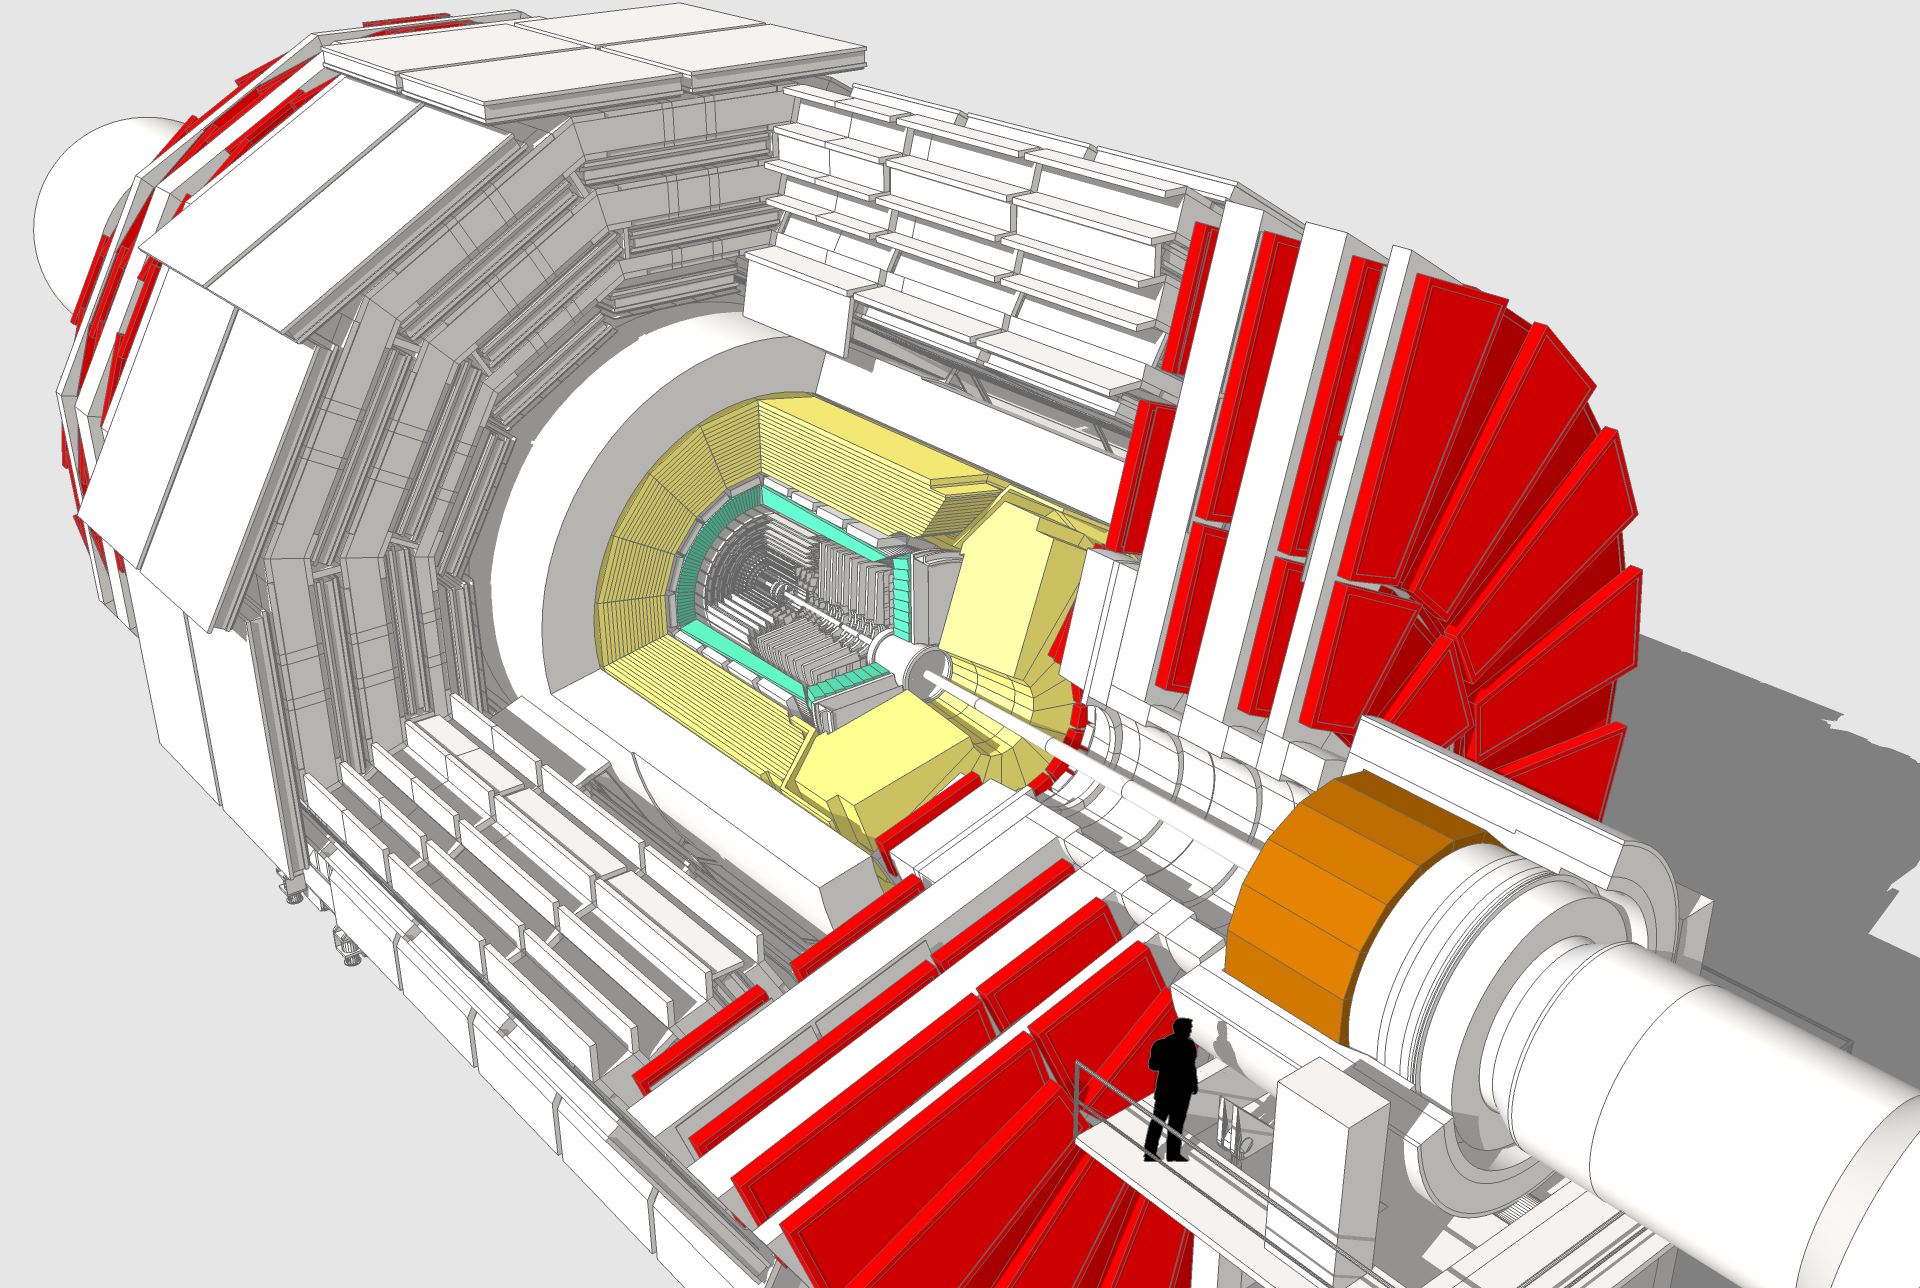
\includegraphics[width=1\textwidth]{figures/cmsDetectorBasic.png}
	\caption{Cut-away view of the entire CMS detector.  Closest to the proton-proton interaction point is the 
		silicon tracker, followed by the electromagnetic calorimeter, then the hadronic calorimeter, and the 
	magnet.  The muon detectors are located in the magnet iron return yoke.}
	\label{fig:layersOfCMS}
\end{figure}

\section{The Silicon Tracker}
\label{sec:siTrackerDescription}
The silicon tracker consisted of silicon pixel and strip detectors whose purpose was to detect and track charged particles 
as they traverse the magnetic field, thereby measuring their radii of curvature.  Then the points where particle tracks 
originated were used to identify interaction vertices.  Closest to the beam axis was the pixel detector, which used 
silicon pixels to measure particles' points of origin and their trajectories up to 15 cm from the $z$ axis.  Surrounding 
the pixel detector was the strip detector, which used silicon strips to measure the radii of curvature of particles up to 
110 cm from the $z$ axis.

%Charged particles produced within the tracker acceptance of $|\eta| < 2.5$ generated an 
%analog signal that was detected and stored in an analog memory until it was readout or discarded.

The pixel tracker was built from $\approx$1 m$^{2}$ of arrays of pixels, each covering 100 $\times$ 150 $\mu$m$^{2}$.  In 
the barrel region ($0 < |\eta| < 1.2$), individual silicon detectors were assembled in three concentric cylindrical shells 
centered on the $z$ axis.  In the endcap region ($1.2 < |\eta| < 2.5$), two layers of pixel detectors were installed in a 
turbine pattern (Figure \ref{fig:pixelTracker}) \cite{pixelCommissioning}.  These provided up to 3 measurements for every 
track, and primarily were used to reconstruct interaction vertices.

\begin{figure}[ht]
	\centering
	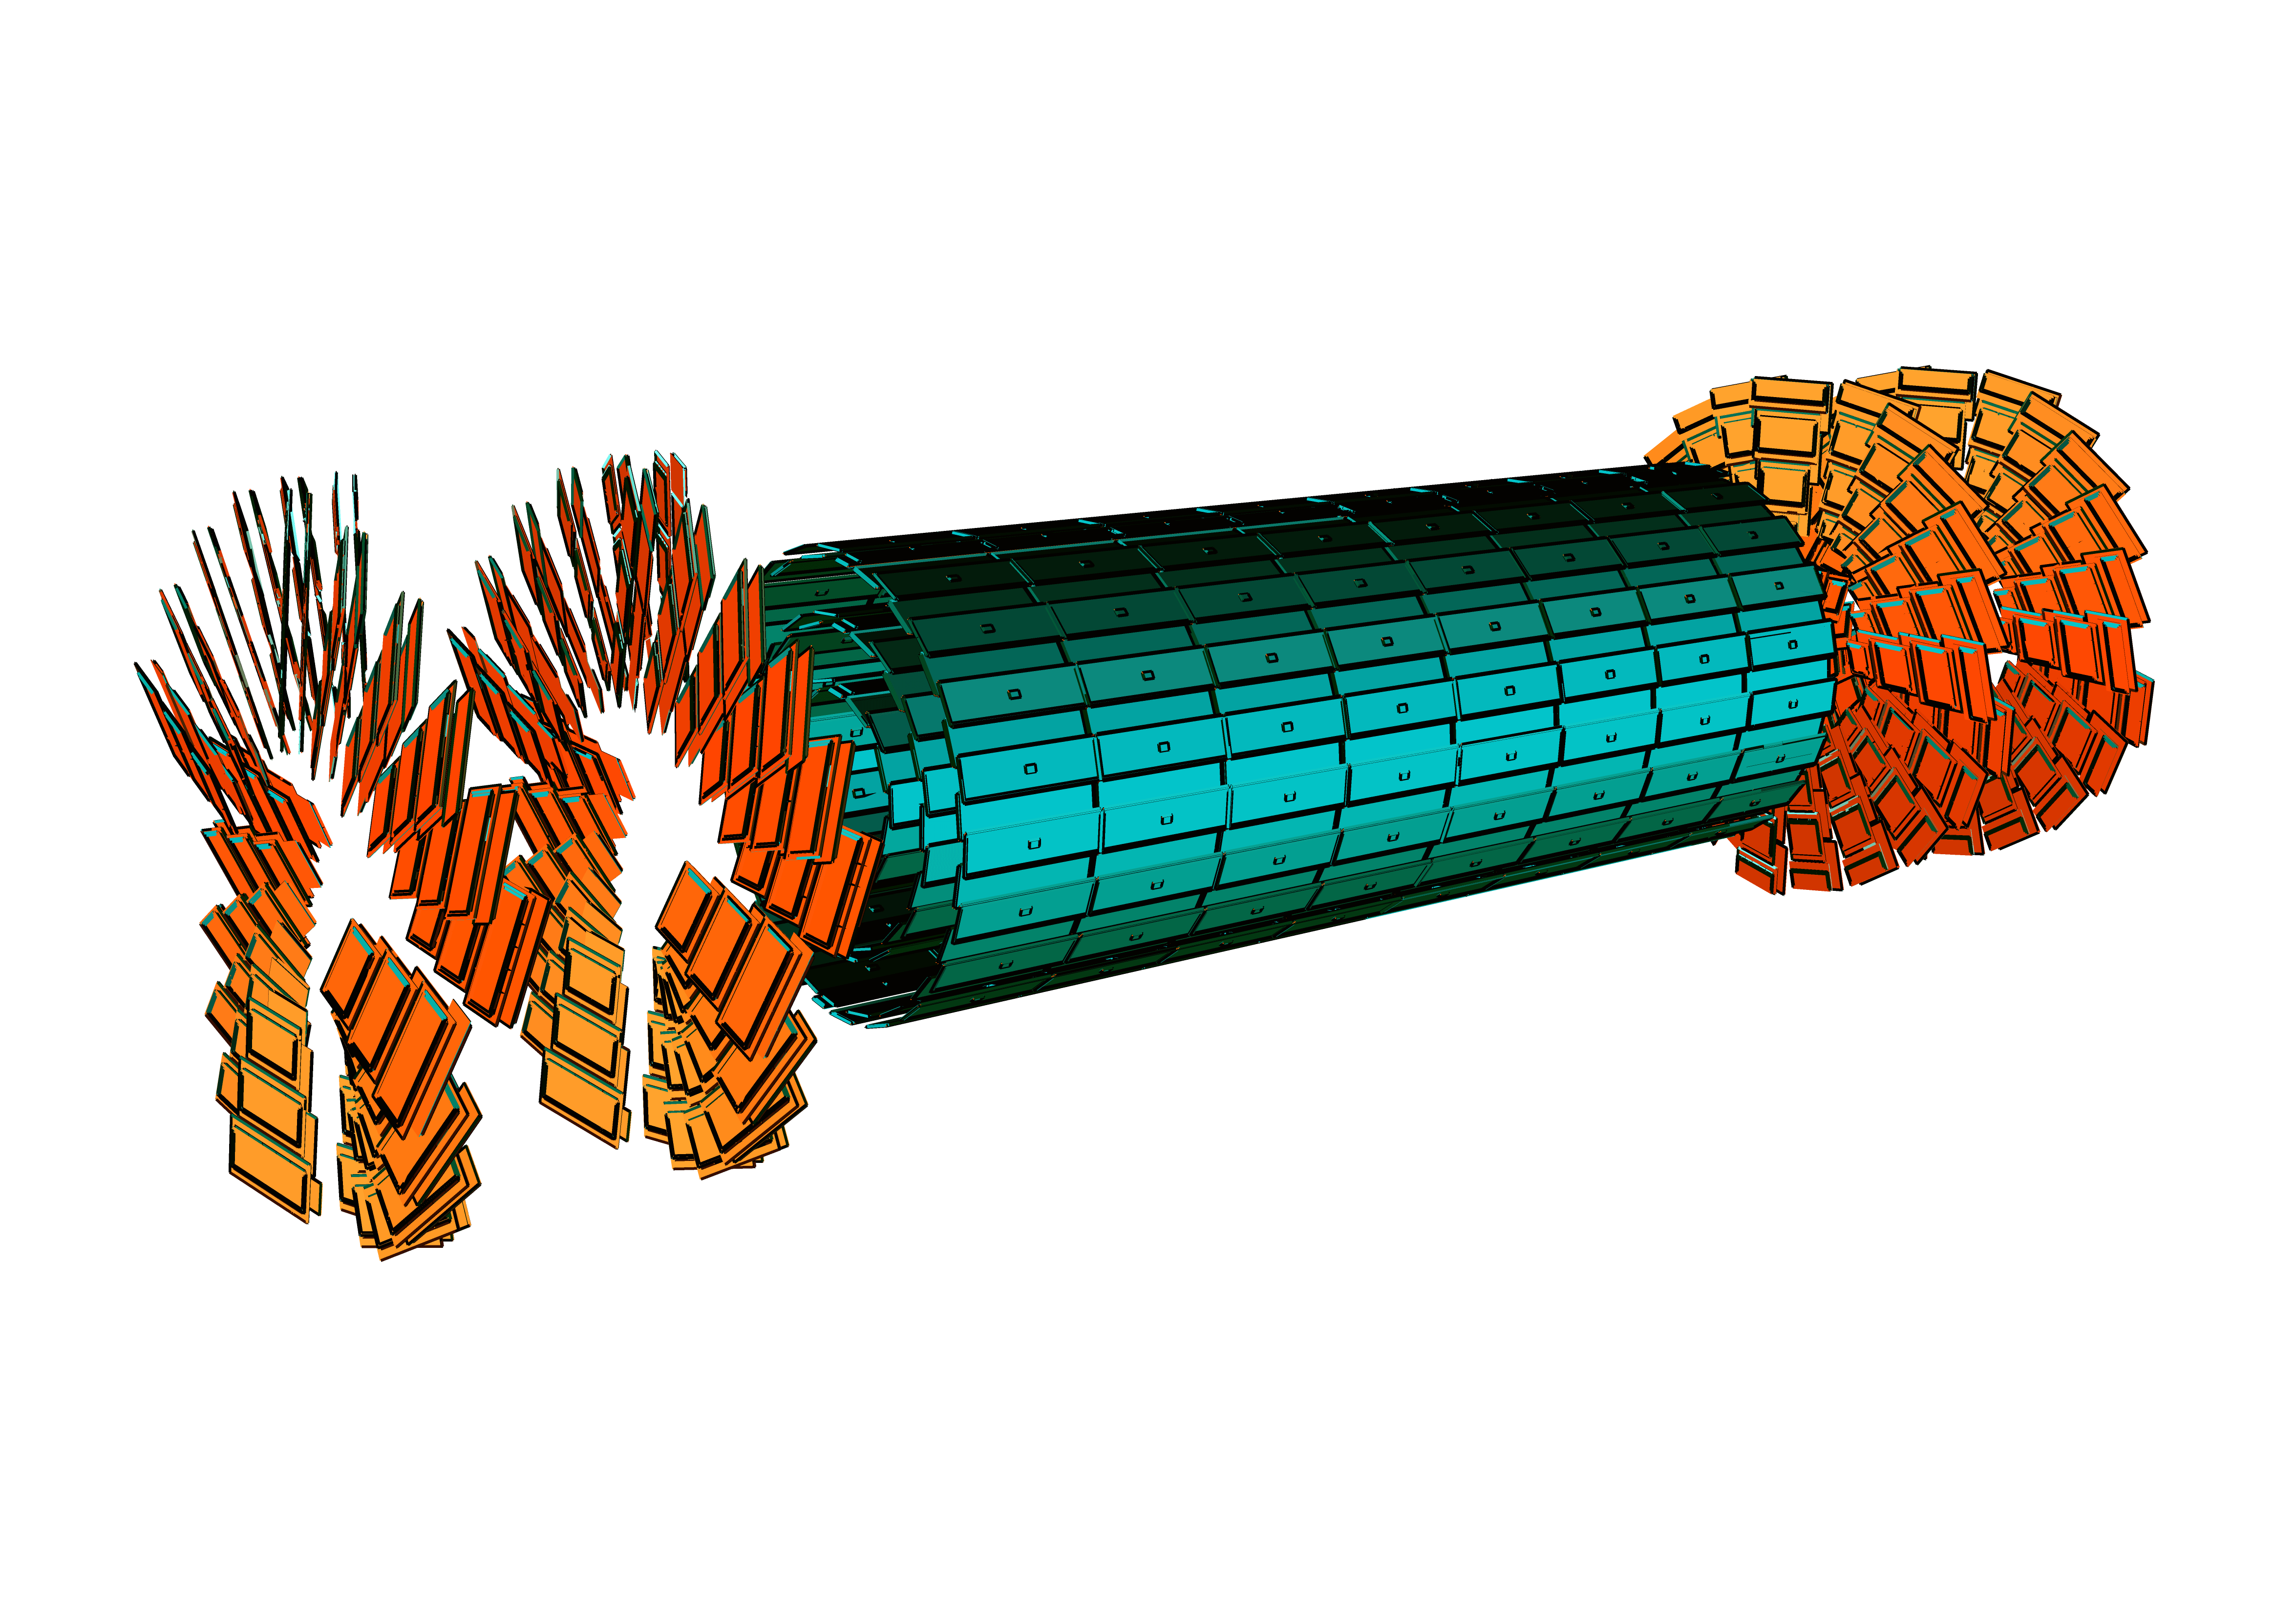
\includegraphics[width=0.8\textwidth]{figures/pixelDetectorSchematic.png}
	\caption{The barrel and endcap sections of the pixel detector.}
	\label{fig:pixelTracker}
\end{figure}

Located outside the pixel tracker, the strip tracker was constructed with 198 m$^{2}$ of silicon divided into arrays of strips, 
and organized into four structures based on $|\eta|$ and distance from the IP.  As the distance from the beam axis increased, the 
strip width increased from 80 to 180 $\mu$m, and the strip length increased from 12 to 16 cm.  
In the barrel region, silicon strips were used to build 10 concentric cylindrical shells.  In the endcap region, silicon 
strips were arranged in 12 disks, as shown in Figure \ref{fig:stripTracker} \cite{cmsTDR}, with some overlap in $|\eta|$ with 
the barrel region silicon strips.  The strip tracker provided between 5 and 14 measurements for every track over a $\sim$1 meter 
distance.

\begin{figure}[ht]
	\centering
	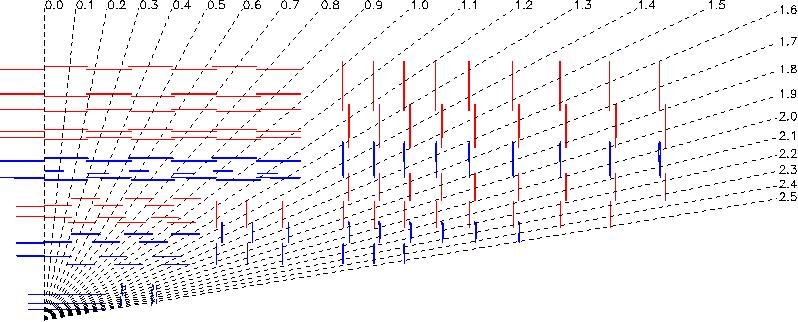
\includegraphics[width=0.8\textwidth]{figures/siliconStripAndPixelDetectorTwoDimView.png}
	\caption{The barrel and endcap sections of the strip detector for $\eta \geq 0.$ and one quadrant of $\phi$.  
	The pixel detector is shown to scale in the bottom left corner.}
	\label{fig:stripTracker}
\end{figure}

The signals from a charged particle traversing the tracker were measured by silicon detector modules that each had arrays of 
individual pixels or strips connected to Read-Out Chips (ROCs).  In the pixel tracker barrel and endcap, each ROC was connected 
to an array of 52 $\times$ 80 individual pixels.  The pixel tracker barrel was divided into silicon detector modules that each had 
16 ROCs.  In the pixel tracker endcap, each turbine blade was divided into 7 silicon detector modules (4 on one face, 3 on the 
other), and each module had between 2 and 10 ROCs.  In total, $\sim$16000 ROCs were connected to 66 million pixels.  Using a 
different type of ROC, 128 individual strips located on the same $\eta$ ring were connected to a ROC to form one strip detector 
module.  The $\eta$ ring structure was used in the strip tracker barrel and endcap for a total of $\sim$15400 modules in the 
strip tracker.

The tracker measured the positions and energies of charged particles at up to 17 points, and as far as 1.1 meters from the beam 
axis.  The track reconstruction algorithms, described later, identified sets of multiple signals as individual particle tracks 
using a Kalman filter and assuming particle trajectories were approximated by a perfect helix.  Along the trajectory of each track, 
the equation of motion of a charged particle in an inhomogenous magnetic field subject to energy losses in silicon was solved 
numerically.  Finally, the particle's $\pt$ was extracted from the numerical solution.

The tracker performance depended on the number and momenta of the charged particles in a collision event.  In events where two leptons 
and jets were reconstructed from tracks that pointed to one vertex, the vertex's position was measured with a resolution better than 
12$\mu$m in any direction \cite{trackerPerformanceInCollisions}.  
The tracker measured charged particle momenta by measuring the radius of curvature of charged particle tracks; thus 
the $\pt$ resolution degraded with increasing $\pt$.  For muons with $20 < \pt < 100$ $\GeV$, the 
tracker measured the $\pt$ of barrel region muons with a resolution of 1.3\% to 2.0\%, and measured the $\pt$ of endcap muons 
with a resolution of 6\% or better \cite{muonRecoFirstCollisions}; higher $\pt$ muons were measured with a worse $\pt$ resolution.  
Charged hadrons that did not undergo a nuclear interaction in the tracker were measured with a $\pt$ resolution similar that of a 
muon.  Accounting for the $\eta$-dependent tracker material budget of 0.18 to 0.56 nuclear interaction lengths, the tracker measured 
the $\pt$ of all charged hadrons with $10 < \pt < 100$ $\GeV$ with a resolution of 3.3\% or better in the barrel, and 20\% or better 
in the endcap \cite{trackerPerformanceInCollisions}.  Electrons were detectable as tracks if they had $\pt > 0.4$ $\GeV$ and 
$|\eta| < 2.5$, but their $\pt$ resolution was significantly worse than that of charged hadrons or muons due to multiple scattering 
and bremsstrahlung.  The tracker measured the $\pt$ of electrons with $10 < \pt < 100$ $\GeV$ with a resolution of between 6\% and 
27\% of $\pt$ in the barrel, and between 20\% and 50\% of $\pt$ in the endcap.

To measure the position of the interaction vertex and charged particle momenta with these resolutions, the alignment and momentum 
response of the tracker were measured before the start of data taking with cosmic ray muons.  The alignment is the position of the 
pixel and strip trackers relative to the calorimeters and muon detectors, and was measured to determine the absolute positions of 
interaction vertices.  The magnitudes of signals generated by charged particles in the pixel and strip detector modules vary with 
$\pt$, and the response of each module versus $\pt$ was measured to identify variations in the tracker measurements versus $\eta$ 
and $\phi$.  During collisions, $Z \rightarrow \mu\mu$ events and cosmic ray muons were used to monitor and recalibrate the tracker 
alignment and momentum response.

In the reconstruction, charged leptons and hadrons were distinguished from photons and neutral hadrons using tracks found in the 
tracker.  Tracks that extrapolated to energy deposits found in the electromagnetic calorimeter (ECAL) or hadronic calorimeter (HCAL) 
were identified as electrons or charged hadrons, respectively.  Tracks found in the silicon tracker that extrapolated to tracks found 
in the muon detectors were identified as muons.


\section{The Electromagnetic Calorimeter}
\label{sec:ecalDescription}
Surrounding the silicon tracker was the electromagnetic calorimeter (ECAL), which detected photons, and distinguished
electrons and positrons ($e^{\pm}$) from other charged particles.  
The ECAL is an absorption calorimeter built from homogeneous, scintillating lead-tungstate (PbWO$_{4}$) crystals.  
In response to incident photons and $e^{\pm}$, the ECAL crystals emitted visible light in amounts proportional to 
the incident particle energies.  The ECAL measured the energies of photons and $e^{\pm}$ that had $0 < |\eta| < 3.0$ by 
measuring the amount of visible light produced by PbWO$_{4}$ crystals.

The ECAL contained 75848 crystals \cite{ecalPerformanceInCollisions} divided into barrel and endcap regions.  In the 
barrel region ($0 < |\eta| < 1.479$), 61200 
crystals with $\sim$26 radiation lengths\footnote{On average the energy of a relativistic $e^{\pm}$ decreases by $e^{-1}$ after 
travelling through one radiation length of material.} of PbWO$_{4}$ were arranged in a cylindrical shell.  The front face of 
each crystal measured 2.2 $\times$ 2.2 cm$^{2}$, and was 19 cm away from the outer most silicon tracker layer.  
In the endcap region ($1.479 < |\eta| < 3.0$), 14648 crystals (half in each 
endcap) with $\sim$25 radiation lengths of PbWO$_{4}$ were installed in a disk.  The front face of endcap crystals measured 2.86 
$\times$ 2.86 cm$^{2}$, and was located behind 3 radiation lengths of lead and silicon that constituted the preshower detector.  
The preshower detector improved the spatial and energy resolution with which electromagnetic showers were studied in the 
endcap.  A partial view of the ECAL barrel, endcap and preshower detectors is shown in Figure \ref{fig:ecalEBEEandES} \cite{ecalTDR}.

%RESUME HERE


\begin{figure}[ht]
	\centering
	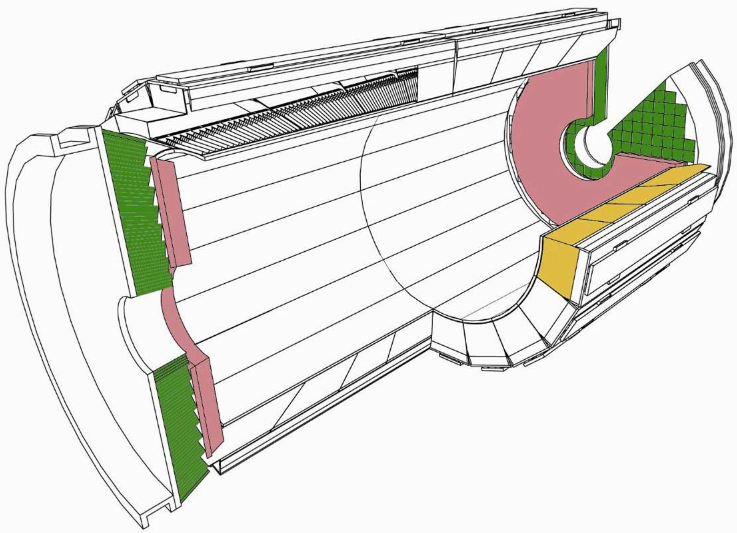
\includegraphics[width=0.8\textwidth]{figures/ecalBarrelEndcapAndPreshower.png}
	\caption{The ECAL barrel, endcap and preshower detectors.}
	\label{fig:ecalEBEEandES}
\end{figure}

Photons and electrons that impinged on the ECAL interacted with lead-tungstate nuclei, causing a scintillation 
signal to be emitted that was detected with avalanche photodiodes in the barrel, and vacuum phototriodes in the 
endcap.  The density of PbWO$_{4}$, 5.4 $\frac{gm}{cm^{3}}$, 
was sufficiently high that the scintillation signal was usually fully contained in a 3 $\times$ 3 crystal 
grid centered on the most energetic crystal.  PbWO$_{4}$ was chosen because the scintillation signal was fast - 
more than 80\% of the scintillation light was emitted in $\sim$20 ns - as required by the 40 MHz pp collision rate.  
The scintillation signal was amplified and measured by photodetectors to determine the energy of incident 
photons and electrons.  Based on real collision data, the ECAL measured the energies of electrons from $Z \rightarrow ee$ 
decays ($\Et \approx 45 \GeV$) with a resolution better than 2\% for $|\eta| < 0.8$, and between 2\% and 5\% elsewhere.  
At a slightly lower $\Et$ scale in real collision data, the ECAL measured the energies of photons from $Z \rightarrow \mu\mu\gamma$ 
decays with a resolution of 2.5\% in the barrel, and 4.7\% in the endcaps \cite{ecalPerformanceInCollisions}.

To measure photon and electron energies with similar precision across the entire detector, the ECAL crystals were 
monitored and calibrated during data taking using several techniques.  Every 40 minutes each ECAL crystal was illuminated 
with light from blue and green lasers to monitor the crystal transparency.  Every week laser data 
was used to calculate new crystal correction factors, which corrected the changes in crystal transparency 
since the previous week.  Photons from $\eta \rightarrow \gamma\gamma$, and electrons from 
$W \rightarrow e\nu$ and $Z \rightarrow e^{+}e^{-}$ were used to validate the weekly transparency corrections.

To compliment the transparency corrections, additional corrections were applied to ECAL crystals 
to calibrate their responses based on the arrival times and energies of reconstructed particles.  Relative energy 
and arrival time corrections for each crystal were calculated using methods described elsewhere \cite{eGammaMonitCalib2011}, and 
were applied to normalize the the responses of all crystals, in terms of energy and time, to the same value.  Then 
absolute energy scale corrections were derived using electrons from $Z \rightarrow e^{+}e^{-}$ events, and applied 
to calibrate each crystal's energy response to the true $Z$ boson mass.  New arrival time corrections were applied 
every month, and new energy corrections were applied once in September 2015.

During particle reconstruction energies measured by individual ECAL crystals were grouped into dynamically 
sized superclusters (SCs) with at least 15 crystals.  The SC size was allowed to vary in $\eta$ and $\phi$ to capture 
bremsstrahlung photons produced when $e^{\pm}$s traversed the silicon tracker.  In the subset of SCs that were isolated 
from HCAL energy deposits, each $e^{\pm}$ was identified as a SC that geometrically matched a reconstructed track 
trajectory, and each photon was identified as a SC not matched to any track.


\section{The Hadronic Calorimeter}
\label{sec:hcalDescription}
Surrounding the ECAL was the hadronic calorimeter (HCAL), which detected charged and neutral hadrons.  The 
HCAL is a sampling calorimeter constructed with 17 layers of 3.7 mm thick scintillating plastic tiles separated by 
17 layers of 5 cm thick metal absorber plates.  In the barrel 
region ($0 < |\eta| < 1.4$), absorber plates and scintillating tiles were organized into 2304 towers, each 
covering a 5 $\times$ 5 grid of ECAL barrel crystals.  In the endcap region ($1.3 < |\eta| < 3.0$), absorber 
plates and scintillating tiles were assembled into 2304 towers (1152 per endcap), each covering 
a 5 $\times$ 5 grid of ECAL endcap crystals.

Hadrons that impinged on the HCAL showered in metal absorber layers, and in $\sim$10 ns produced scintillation 
light in the plastic tiles.  Optical fibers transmitted the scintillation light to hybrid photodiodes, 
which measured the scintillation light to determine the energies of incident hadrons.  The HCAL was used in 
combination with the tracker, ECAL, and muon detectors to measure the energy of jets.  After calibrating the 
HCAL and the other sub-detectors, the energy of jets with $\pt > 40\GeV$ and $|\eta| < 1.3$ was measured with 
a resolution of 16\% or better \cite{jetResolutionInCollisions}.

To measure hadron energies with similar precision across the whole detector, the amount of light measured in scintillating tile towers 
was monitored and calibrated before and during 2015 collisions.  Before collisions, a radioactive source 
with known radioactivity was lowered into the HCAL, and the amount of scintillation light produced by each 
tower was used to calibrate each tower's response.  Once collisions began, a laser system 
monitored the efficiency of light transmission from the scintillator tiles to the photodetectors.  
From laser transparency data, relative calibrations were derived that normalized the energy response of all towers 
to the same level.  The absolute energy calibration was determined in events where a jet recoiled off a photon, or 
a leptonically decaying Z boson.  There, the absolute hadronic energy 
scale was calibrated relative to the electromagnetic or muonic energy scale derived from $Z \rightarrow \ell\ell$ 
and $Z \rightarrow \mu\mu\gamma$ events.  Finally, the precision of the absolute hadronic energy scale calibration 
was improved using dijet resonances like $W/Z \rightarrow jj$.

During particle reconstruction the energy measured by each HCAL tower was treated as the basic unit of HCAL energy.  
Each reconstructed hadron contained at least one HCAL energy deposit, and potentially one or more ECAL energy 
deposits.  Reconstructed tracks that extrapolated to the $(\eta,\phi)$ positions of HCAL energies were identified 
as charged hadrons, while HCAL energies that did not match any track were identified as neutral hadrons.


\section{The Muon Detectors}
\label{sec:muonDetectorsDescription}
Interspersed among layers of the magnet iron return yoke were gas ionization chambers used to detect muons.  Muons 
that traversed the chambers ionized charge along their trajectories, and the ionized charges drifted to 
anodes and cathodes.  The muon detectors measured the momenta, trajectories, and arrival times of muons with $0 < |\eta| < 2.4$ by 
measuring the amount of charge collected by the anodes and cathodes.  Since the muon detectors were located 13 light-ns 
or further from the IP, the muon detectors measured each muon's arrival time to identify the collision event that produced it.

The muon barrel and endcap sections, shown in Figure \ref{fig:muonBarrelAndEndcapDetectors}, used three types of 
gas ionization detectors to measure muon kinematic quantities.  In the barrel region ($0 < |\eta| < 1.2$), 
drift tubes (DTs) and resistive plate chambers (RPCs) measured muon momenta, trajectories, and arrival times.  In 
the endcap region ($1.2 < |\eta| < 2.4$), RPCs and cathode strip chambers (CSCs) measured the same quantities.

\begin{figure}[ht]
	\centering
	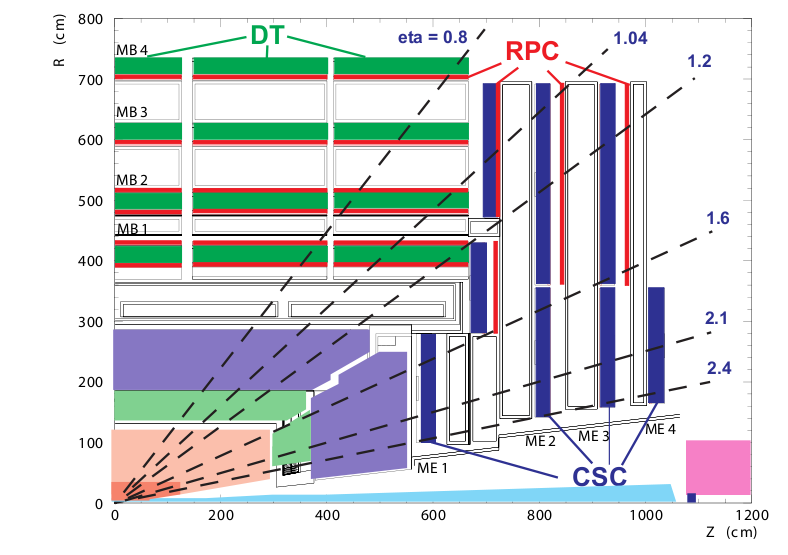
\includegraphics[width=0.8\textwidth]{figures/muonDetectorLayout.png}
	\caption{The barrel and endcap sections of the muon detectors for $\eta \geq 0.$ and one quadrant of $\phi$.  Shown 
		between the muon detectors and the interaction point are the magnet solenoid and return yoke, the HCAL, the ECAL, 
		and the silicon tracker.}
	\label{fig:muonBarrelAndEndcapDetectors}
\end{figure}

The DTs were organized into 5 wheels, each with 4 radial layers called stations, and 12 $\phi$ segments per 
station that each covered 30 degrees in $\phi$.  Each DT chamber measured muon trajectories using 8 planes of 
drift tubes in r-$\phi$, and 4 planes of drift tubes in r-z\footnote{There were no r-z planes of drift tubes in 
the outermost station}.  Using these planes, in 2015 collisions each DT station measured muon trajectories 
with a resolution better than 300$\mu$m in any direction, and measured muon arrival times with a resolution of 2 ns \cite{cmsMuonRecoRunTwo}.  

In the endcap, CSCs were installed in four disks that faced the interaction point.  
The disks were segmented into several radial layers (rings of different radii, 'stations'), as shown in Figure 
\ref{fig:muonBarrelAndEndcapDetectors}, that each contained 18 or 36 chambers, and each chamber had 6 planes of CSC detectors.  
These chambers measured muon trajectories with a resolution better than 150 $\mu$m in any direction, and measured muon arrival 
times with a resolution of 3.2 ns.

In the barrel and endcap for $|\eta| < 1.9$, the RPCs measured muon arrival times with a resolution better than 
2 ns.  RPC measurements were used by the trigger system to identify the collision event that produced each muon \cite{cmsMuonRecoRunTwo}.

The muon detectors complimented measurements made by the tracker, and improved the $\pt$ resolution of high $\pt$ muon 
measurements relative to the tracker only performance.  Thanks to the 3.8 $\unit{T}$ magnetic field, the tracker measured 
muon momenta in the $\pt <$ 200 $\GeV$ phase space with a resolution better than the muon detectors by a factor of 3 or 
more.  As the muon $\pt$ increased above 200 $\GeV$, a muon's trajectory through the tracker approached a straight line path, 
and the tracker momentum resolution degraded.  However, the muon detectors measured the curvature of muon tracks over several 
meters, and as a result measured the $\pt$ of $\pt > 200$ $\GeV$ muons with a better resolution than the tracker.  Based on 
cosmic ray muons detected in 2015, the combined tracker and muon detector system measured the $\pt$ of barrel region muons 
that had $200 < \pt < 400 \GeV$ with a resolution of 3.5\% or better \cite{cmsMuonRecoRunTwo}.

The muon detectors measured curved tracks that were used in muon reconstruction.  Muons produced outside the silicon tracker 
were identified as individual tracks in muon detectors, while muons produced within the silicon tracker were identified 
as silicon tracker tracks whose trajectories extrapolated to muon detector tracks.


\section{The Trigger System}
\label{sec:triggerDescription}
In 2015 the rate of pp collision events delivered by the LHC was several orders of magnitude greater than the 
rate that CMS could process collision event data into reconstructed particles.  The LHC collided two proton bunches 
at a rate of 40 MHz, and in nearly every collision $\gtrsim$1 $\GeV$ of energy was detected in CMS.  Due to the large cross 
section of QCD multijet processes and leptonically decaying heavy quark processes (Figure \ref{fig:smProductionXsxns}), CMS 
detected $\sim10^{6}$ collision events per second with energetic charged leptons or hadronic jets.  In 2015 
CMS was able to readout all detector information and subsequently reconstruct particles in only $\sim10^{3}$ 
collision events per second, so a two level trigger 
system selected events during collisions (online) that were reconstructed for physics analyses and detector calibration.

\begin{figure}[h]
	\centering
	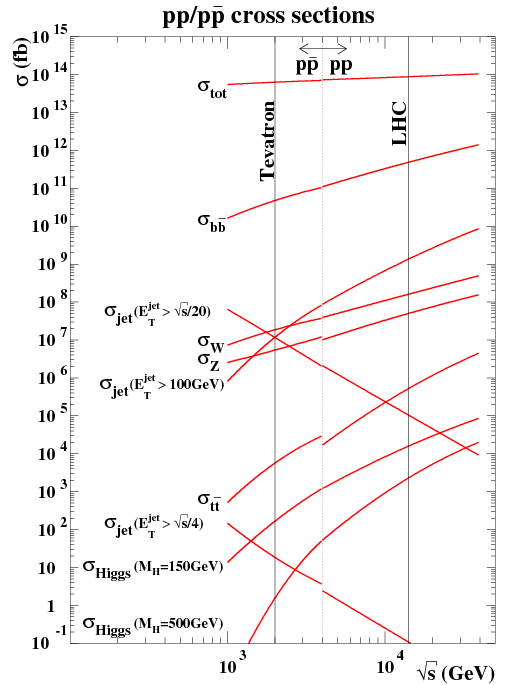
\includegraphics[width=0.6\textwidth]{figures/lhc_and_tevatron_cross_sections_2006.png}
	\caption{Production cross sections at the LHC and Tevatron as a function of center of mass energy.  Each cross section divided by $10^{5}$ yields 
	the approximate production rate in events per second in 2015 at the LHC.}
	\label{fig:smProductionXsxns}
\end{figure}

The Level-1 (L1) trigger system searched for collision events with photons, charged leptons, hadronic 
jets or neutrinos.  After every collision event, data from the ECAL, the HCAL and the muon detectors was used to build trigger 
primitive objects that represented photons, muons and other particles.  In $\sim$1 $\mu$s these objects, 
distinguished by $\Et$ values and $(\eta, \phi)$ coordinates, were built and sent to the L1 logic system located 
$\sim$20 m from CMS.  Implemented in programmable hardware like Field Programmable Gate Arrays, the L1 
logic system ran $\sim$200 algorithms in less than 1 $\mu$s, and identified trigger primitive objects passing $\Et$ 
and $|\eta|$ selection criteria.  Approximately 80000 events per second were found with at least one trigger 
primitive object passing selection criteria, and these events were processed by the second level trigger.  

The second level, or High Level, trigger (HLT) selected events for offline reconstruction and subsequent 
use in physics analyses and detector calibration analyses.  The HLT began by transferring data from all 
sub-detectors to multi-core processors running the HLT software.  
A fast, simplified version of the full offline particle reconstruction software was run in small 
regions where L1 trigger algorithms had fired.  Then, $\sim$400 different selection algorithms, running in 
parallel, applied selection criteria ($\Et$, $|\eta|$, etc) to locally reconstructed particles 
to select energetic photons, charged leptons, jets, and neutrinos.  About 1000 events per second passed at least 
one selection algorithm, and these events were stored offline for subsequent reconstruction using the entire event 
information.  Offline, events were selected based on the kinematics of reconstructed electrons, muons, and jets.  
The particle reconstruction algorithms and selection criteria are described in the next chapter.

%Considering events selected by any HLT algorithm, during 2015 pp collisions the rate of data written to 
%permanent storage was $\lesssim 0.5$ gigabytes per second.

